% CAPITOLO LITERATURE REVIEW
\newpage
\section{Literature Review}
\label{section:literatureReviewChapter}
This chapter provides an in-depth overview of the field of generative modelling. It lays out the theoretical background of the thesis, beginning with a general explanation of how GANs works and then exploring some useful theoretical concepts.

\subsection{GAN}
The innovative concept of Generative Adversarial Networks (GANs) was first introduced in 2014 by Goodfellow and his colleagues from the University of Montreal~\cite{GANGoodfellow}. GANs are a type of deep learning model that has the ability to generate new content, such as text or images, based on a given dataset. GANs have been the focus of significant research in recent years and have made significant contributions to the field of computer vision. The technology has advanced in areas like generating realistic images, transforming images, modifying facial features, and similar topics, but also in other areas such as music generation.\\
Before the advent of GANs, machine learning algorithms were highly effective in recognising patterns in existing data and could be utilised for tasks like classification and prediction. However, generating new data presented a challenge for these algorithms. The solution proposed in the GAN paper leverages the strengths of machine learning algorithms — their ability to classify and predict – to overcome their weaknesses in generating new content.\\
The approach involves setting two algorithms against each other in a kind of competition, leading to a continuous process of improvement. This approach has proven to be highly effective in generating new, diverse content and has been widely adopted in the field of deep learning.
Before diving into the intricacies of GANs, it is essential to understand how these networks work. A widely used analogy can provide a clearer insight.\\
\\
Imagine there is an art forger and an art authenticator. The forger's goal is to produce a counterfeit piece of art that the authenticator will consider genuine. The authenticator is trained to recognise genuine art by examining real pieces, while the forger learns by creating art that is then evaluated by the authenticator. In GANs, the forger is the generator, which strives to produce examples that are indistinguishable from the real data in the training set, thus trying to fool the discriminator. On the other hand, the discriminator acts as the art authenticator, evaluating the authenticity of the generated pieces. These two networks are in a constant battle, each trying to outsmart the other. As the generator improves in creating realistic data, the discriminator needs to enhance its capability in detecting fake examples. Similarly, as the discriminator becomes better in differentiating true from false, the generator must strive to generate even more convincing fake data. The most critical aspect of this architecture is that the generator has no direct connection to the actual image, its only way to learn is through its interaction with the discriminator~\cite{GeneratingNewRealityBook}. Fig.~\ref{fig:GAN architecture} illustrates a simple GAN architecture based on the analogy.
\begin{figure}[h!]
\centering
  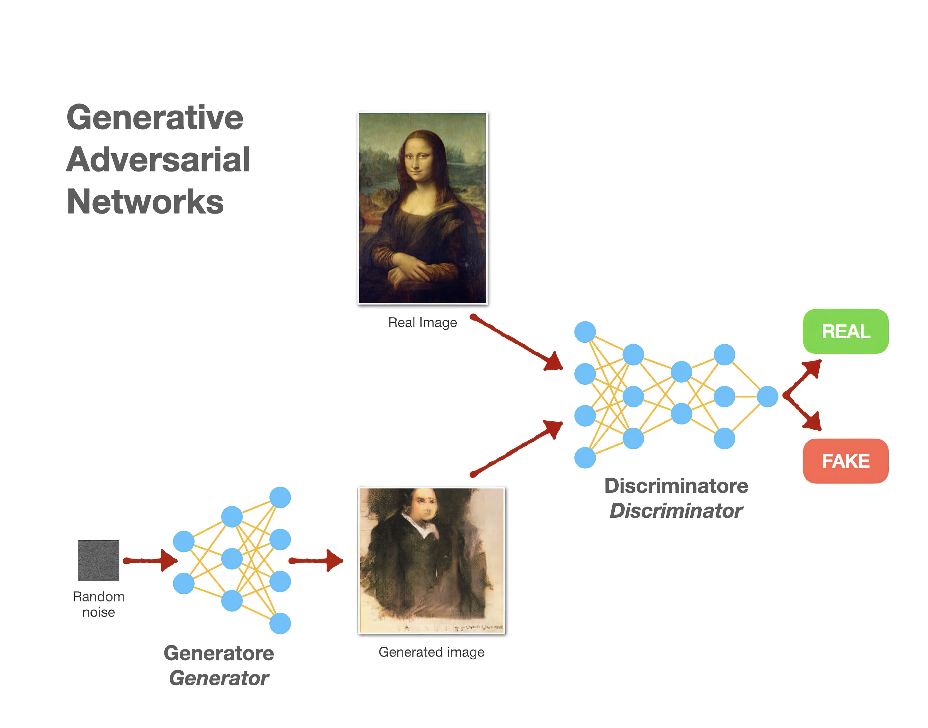
\includegraphics[scale=0.5]{figures/GANs-ex-art.png}
  \caption{Example of a GAN architecture}
  \label{fig:GAN architecture}
\end{figure}

\subsubsection{GAN structure and training}
\noindent A GAN has a similar structure to that of an autoencoder, where the discriminator serves as the encoder. However, instead of producing an encoded representation, it only outputs whether the input is real or fake. On the other hand, the generator acts like the decoder and takes in random data from the latent space, learning to generate new content that can trick the discriminator into thinking it is real. Both the generator and discriminator are trained in a competitive manner, with the generator striving to maximise the error of the discriminator and the discriminator trying to minimise it.\\
\\
The generator and the discriminator are two distinct deep neural networks. The generator is a function G that takes random noise vector $z$ as inputs and maps them to the data space, producing a set of synthetic samples. These samples are fed into the discriminator network D, together with the real samples $x$. This network outputs a single scalar that represents the probability that the sample came from the real data distribution rather than the synthetic data distribution. Therefore, the discriminator learns to use traditional supervised learning techniques, dividing inputs into two classes (real or fake).\\
The GAN training process is a two-player that involves updating the weights of the generator and discriminator networks using gradients computed from the loss function. The loss function, also called cost function, in a GAN is designed to quantify the difference between the generated data and the real data. The objective is to find the balance between the generator and discriminator losses, where the generator loss represents the ability of the generator to produce realistic synthetic data and the discriminator loss represents the ability of the discriminator to distinguish between real and fake data.\\
There are several cost functions that may be used, and they usually differ in terms of the cost function used for the generator.\\
The basic loss function used in GAN is the binary cross-entropy:
\begin{equation}
\label{eq:binariCross-entropy}
L(\hat{y}, y) = [y \times \log (\hat{y}) + (1-y)\times \log (1-\hat{y})]
\end{equation}
where $y$ represent the original data and $\hat{y}$ the generated one. In training, the discriminator assumes $y=1$ for real data, while for the generated data it is set: $\hat{y} = D(x)$. Substituting this information in equation~\ref{eq:binariCross-entropy} it can be obtained the discriminator loss: 
\begin{equation}
    L(D(x),1)=\log(D(x))
\end{equation}
For the generator's output data it is assumed $y = 0$, because it outputs fake data, and $\hat{y} = G(D(z))$ for the generated data, where $z$ is a random noise vector sampled from a noise distribution $p_z(z)$ (e.g., uniform or Gaussian distribution). Therefore, the loss for the generator is:
\begin{equation}
    L(D(G(z)),0) = \log(1 - D(G(z)))
\end{equation}
To obtain the total discriminator loss the two above equations have to be combined and maximised:
\begin{equation}
L^{(D)}=\max [\log (D(x)) + \log(1-D(G(z)))]
\end{equation}
The generator has to fool the discriminator, hence it has the opposite goal, therefore to obtain its loss function its minimum has to be calculated:
%is obtaining by computing the minimum:
\begin{equation}
L^{(G)}=\min [\log (D(x)) + \log(1-D(G(z)))]
\end{equation}
The loss function is designed to encourage the generator to produce realistic synthetic data and the discriminator to distinguish between real and fake data with high accuracy.
\\
The interdependence of each player's cost on the other player's parameters, along with the lack of control over the other player's parameters, makes this scenario more accurately described as a game rather than an optimisation problem. 
%The solution of this game is the \textit{Nash equilibrium}.
The loss function in a GAN is an important component of the training process, as it determines the quality of the generated data and the ability of the discriminator to accurately distinguish between real and fake data. 
\\
\noindent The training process of GANs is a zero-sum game in which the objective function of this minimax optimisation problem is:
\begin{equation}
\label{eq:minimax obj function}
    \min \max V(D,G) = \min_G \max_D \mathbb{E}_{x \sim p_{data}(x)}[\log D(x)]+\mathbb{E}_{z \sim p_z(z)}[\log (1- D(G(z)))]
\end{equation}
where $x$ is a real image from the true data distribution $p_{data}$, and $z$ is a noise vector sampled from the noise distribution $p_z$. $\mathbb{E}_x$ and $\mathbb{E}_z$ denote the expected log likelihood from the different outputs of both real and generated images.

\noindent In training a GAN, it is important to ensure that both the generator and discriminator models are developed in a balanced manner. The success of the GAN largely depends on the alignment of the real and generated distributions, and this can only be achieved if neither of the models is overly dominant.
In addition to train the generator and the discriminator, the errors on their outputs are backpropagated into the models as gradients of the loss functions, as shown in Fig.~\ref{fig:GAN architecture w loss}. These loss functions are used to guide the learning process and ensure that the generator produces high-quality samples.
\begin{figure}[!ht]
\centering
  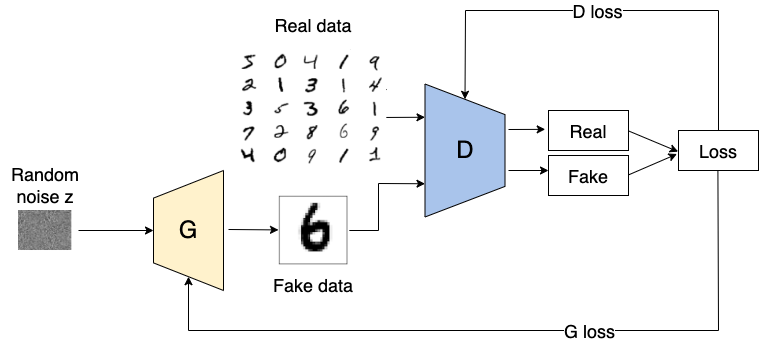
\includegraphics[scale=0.45]{figures/gan-architecture.png}
  \caption{Architecture of a GAN. The generator and the discriminator are synchronously trained.}
  \label{fig:GAN architecture w loss}
\end{figure}
If the discriminator is too good at identifying fake versus real images early in the training process, the generator may struggle to produce convincing fake images, making it difficult for the two models to improve. If the generator is successful in fooling the discriminator, the loss will backpropagate through the discriminator network to improve its performance. On the other hand, if the discriminator effectively distinguishes between fake and real samples, the loss will backpropagate through the generator network to improve its ability to generate samples that are similar to real samples.
The update rules for the discriminator and the generator are the shown equation~\ref{eq:update rule discriminator} and~\ref{eq:update rule generator} respectively. The weights of each model are represented by $\theta_d$ and $\theta_g$, respectively, and $m$ represents the total number of samples in a batch used to test the models before updating them. Algorithm~\ref{alg:training optimisation} optimises Eq.~\ref{eq:minimax obj function} as show by~\cite{GANGoodfellow}.
\begin{algorithm}
\caption{Minibatch stochastic gradient descent training of generative adversarial nets. The number of steps to apply to the discriminator, $k$, is a hyperparameter.}\label{alg:training optimisation}
\begin{algorithmic}
\For {number of training iteration}
    \For {$k$ steps }
         \Statex\begin{itemize}
         \setlength{\itemindent}{.2in}
             \item Sample minibatch of $m$ noise samples $\{ \mathbf{z}^{(1)}, ..., \mathbf{z}^{(m)}$ from noise prior $p_g(\mathbf{z})$
             \item Sample minibatch of $m$ examples $\{ \mathbf{x}^{(1)}, ..., \mathbf{x}^{(m)}$ from data generating distribution $p_{pdata}(x)$.
             \item Update the discriminator by ascending its stochastic gradient: 
                \begin{equation}
                \label{eq:update rule discriminator}
                    \nabla_{\theta_d}\frac{1}{m}\sum_{i=1}^m [ \log D(x^{(i)}) + \log (1 - D(G(z^{(i)})) ]
                \end{equation}
         \end{itemize}
    \EndFor
    \begin{itemize}
     \setlength{\itemindent}{.2in}
        \item Sample minibatch of $m$ noise samples $\{ \mathbf{z}^{(1)}, ..., \mathbf{z}^{(m)}$ from noise prior $p_g(z)$. 
        \item Update the generator by descending its stochastic gradient:
        \begin{equation}
        \label{eq:update rule generator}
            \nabla_{\theta_g}\frac{1}{m}\sum_{i=1}^m [ \log (1 - D(G(z^{(i)})) ]
        \end{equation}
    \end{itemize}
\EndFor
\end{algorithmic}
The gradient-based updates can use any standard gradient-based learning rule.
\end{algorithm}
%In particular, the generator loss is typically formulated to maximize the probability that the discriminator misclassifies the generated samples as real, while the discriminator loss is formulated to accurately distinguish between real and fake samples. By optimizing these loss functions, the generator and discriminator are trained to achieve better performance over time.
%Therefore, it is crucial to establish a balanced relationship between the generator and discriminator models, allowing them to train efficiently and effectively.

%The training algorithm for GANs involves iterative updates to the discriminator and generator through gradient ascent and descent, respectively. The process is summarized in Algorithm 1.
\noindent From a mathematical point of view, if the discriminator gets too good at identifying the samples, this may increase the divergence between the generated expected distribution. In case the generated and the real distributions become too diverse or do not overlap, then the generator will suffer from vanishing gradient loss. \\
The vanishing gradient problem is a critical issue in training deep neural networks. The problem occurs when the gradients of the parameters with respect to the loss become extremely small, making it difficult for the optimizer to update the parameters of the network effectively since they have no effect on the training model. The vanishing gradient problem can lead to slow convergence or complete failure of the training process. The goal is to make the expected and generated distribution match as closely as possible. 
The GAN continues this back and forth process until an equilibrium is reached between the generator and discriminator loss. Over time, the two networks learn from each other and converge to a state where the generator produces samples that are almost indistinguishable from real data, and the discriminator is able to correctly identify which samples are real and which are fake with high accuracy.
 \\
This basic design is referred to as the Vanilla GAN, as it represents the original model from which more advanced GAN architectures have evolved, yet still retaining the two key components of the GAN structure.
% ************************************
% ************************************
\subsection{Wasserstein-GAN}
\label{sec:wgan}
The Wasserstein-GAN, also known as WGAN, is a variant of the Vanilla GAN introduced by Arjovsky et al. in 2017~\cite{wgan}. WGAN aims to improve the generator model's capability of approximating the data distribution of a given training dataset by introducing a different training mechanism. Instead of using a discriminator to classify the generated images as real or fake, WGAN uses a critic that scores the authenticity of an image. It uses the Wasserstein distance (also known as Earth-Mover's distance), which is a metric that quantifies the minimum cost of moving mass from one distribution to another to convert the source distribution $q$ to the target distribution $p$. It is used to measure the distance between the distribution of real data and the distribution of generated data.\\
In WGAN, the discriminator is trained to be a function that outputs a scalar value instead of a probability, and the generator is trained to minimize the Wasserstein distance.\\
One formulation for the Wasserstein distance is:
\begin{equation}
    \label{eq:waaserstein distance}
    W(\mathbb{P}_r , \mathbb{P}_g)= \sup_{f \in \mathcal{F}} \mathbb{E}_{x\sim \mathbb{P}_r}[f(x)] - \mathbb{E}_{x \sim \mathbb{P}_g}[f(x)]
\end{equation}
where $\mathcal{F}$ is defined as the set of 1-Lipschitz function, which are those satisfying $\|f\|_L \leq 1$ where $\| \cdot \|_L$ represents the Lipschitz norm.\\
The WGAN objective function can be formulated as:
\begin{equation}
    \min_G \max_{D \in \mathcal{F}} \mathbb{E}_{\mathbf{x} \sim \mathbb{P}_r} [D(\mathbf{x})] - \mathbb{E}_{\Tilde{\mathbf{x}} \sim \mathbb{P}_g}[D(\Tilde{\mathbf{x}})]
\end{equation}
where $\mathbb{P}_r$ and $\mathbb{P}_g$ are respectively the real and generated distribution, $\Tilde{\mathbf{x}} = G(z)$ with $z \sim p(z)$.
The above formulation needs the critic to be 1-Lipschitz. This condition is ensured by clipping the weights $\mathbf{W}$ of the discriminator to be within a compact range of $[-c ,c]$, where $c$ is a user-defined hyper-parameter. Specifically, each weight $w_{i,j}$ is clipped to this range.\\ \\
%
%
\textbf{WGAN-GP}\\
One step towards stable training of GANs is made by WGAN, however, it may still generate inadequate samples or not converge. The cause of such issues is frequently attributed to the utilization of weight clipping in WGAN, which enforces a Lipschitz constraint on the critic and can result in undesirable behaviour, for example, the convergence of a very deep WGAN critic may often fail. Therefore, to address this issue an alternative to weight clipping to ensure smooth training has been proposed by~\cite{wgan-gp}, which is the Wasserstein GAN with Gradient Penalty (WGAN-GP).
The WGAN-GP method replaces weight clipping with a gradient penalty, introducing an extra loss term that encourages the discriminator to have a gradient with a norm that is near $1$. The resultant optimization problem is given by: 
\begin{equation}
    L = \mathbb{E}_{\Tilde{\mathbf{x}}\sim \mathbb{P}_g}[D(\Tilde{\mathbf{x}})] - \mathbb{E}_{\mathbf{x}\sim \mathbb{P}_r}[D(\mathbf{x})] + \lambda \mathbb{E}_{\hat{\mathbf{x}}\sim \mathbb{P}_{\hat{\mathbf{x}}}} [( \| \nabla_{\hat{\mathbf{x}}} D( \hat{\mathbf{x}}) \|_2 - 1)^2]
\end{equation}
where the first two terms are the original critic loss of the WGAN, while the last term is the gradient penalty, in which $\lambda$ defines the gradient penalty coefficient, $\hat{x}$ is a random sample along the straight line between real and generated samples and $p_{\hat{x}}$ is the distribution of $\hat{x}$.
% ************************************
% ************************************
\subsection{ProGAN}
\label{sec:proGAN}
ProGAN, short for Progressive Generative Adversarial Network, is a deep learning model that was developed to generate high-resolution, photorealistic images. It was introduced by Karras et al. in 2017~\cite{ProGAN}, it is a type of generative model, which means that it can generate new, synthetic images based on the data it was trained on.\\
The main idea behind ProGAN is to use a series of generators and discriminators to generate high-resolution images incrementally, starting from low-resolution images (e.g. 4×4) and gradually increasing the resolution until a high-resolution image is obtained (e.g. 1024×1024). This approach is called progressive growing, and it allows the network to learn the finer details of an image in an incremental manner. The generator starts with a random noise input and generates an image with low resolution, which is then evaluated by the discriminator. The discriminator determines whether the generated image is real or not and provides feedback to the generator, allowing it to improve. \\ \\
%
One of the benefits of ProGAN is that it generates high-resolution images that are photorealistic, which makes it useful for various applications. Additionally, ProGAN is trained on large datasets, which means that it can create diverse and varied images.
Another advantage of ProGAN is its ability to produce images at different resolutions, which allows for a level of control over the generated images. \\
Some of the drawbacks of the progressive growth method in a GAN are the prolonged training time involved in constructing subsequent models at higher resolutions, the need for extra resources in terms of data preparation and storage, and of course the non-negligible computational time.
%
%
%
\subsection{Evaluation metrics}
\subsubsection{xCos}
\label{sec:xcos}
The state-of-the-art face verification models employ a methodology that involves extracting deep features from a pair of face images and subsequently computing the cosine similarity or the L2-distance of the paired features. The determination of whether the two images are of the same person is based on whether the similarity value exceeds a pre-defined threshold value. However, the approach proposed in the paper “xCos: An Explainable Cosine Metric for Face Verification Task”~\cite{xCos} offers a distinctive approach in which the verification result is obtained by the integration of the local similarity map and the attention map. It is based on the insight that humans tend to compare different facial features to determine whether two face images belong to the same individual. \textit{xCos} leverages this understanding to evaluate the similarity of facial features between two images. It is built using a grid-based feature extraction approach, in which each face image is divided into multiple local regions. The facial features of each local region are then extracted and compared with the features of the corresponding regions in the other image. The resulting similarities are then aggregated across all the local regions to compute a final similarity score. It also includes an attention mechanism that identifies the specific facial features that contribute the most to the similarity score. This attention mechanism allows for a more interpretable and explainable verification result, as it highlights the specific facial features that the model is prioritizing. \\ \\
%
The proposed architecture, showed in Fig.~\ref{fig:xCos architecture}, for face recognition consists of a modified CNN backbone and two branches for xCos and identification. The primary responsibility of the CNN backbone is to extract facial features for each identity. To preserve the position information of each feature point, the final flatten and fully-connected layers of the backbone, such as ArcFace~\cite{arcface2018} or CosFace~\cite{cosFace}, are replaced with a 1 by 1 convolution.
On the xCos branch, to compute a patched cosine map $S$ ($\cos_{patch}$), the two feature maps of compared images are element-wise evaluated using cosine similarity.
At the same time, an attention weight map $W$ is generated using the attention mechanism based on the two feature maps. The final xCos similarity value is achieved by performing a weighted sum of the patched cosine map $S$, using the attention weight map $W$.\\
%
The xCos branch is trained using cosine similarity computed by another face recognition model, such as ArcFace. The identification branch flattens the extracted feature and feeds it into another fully connected layer for predicting the identity. The training is stabilised by using a common face recognition loss, such as the one used in ArcFace, which is denoted as $\mathcal{L}_{ID}$.
\begin{figure}[h!]
\centering
  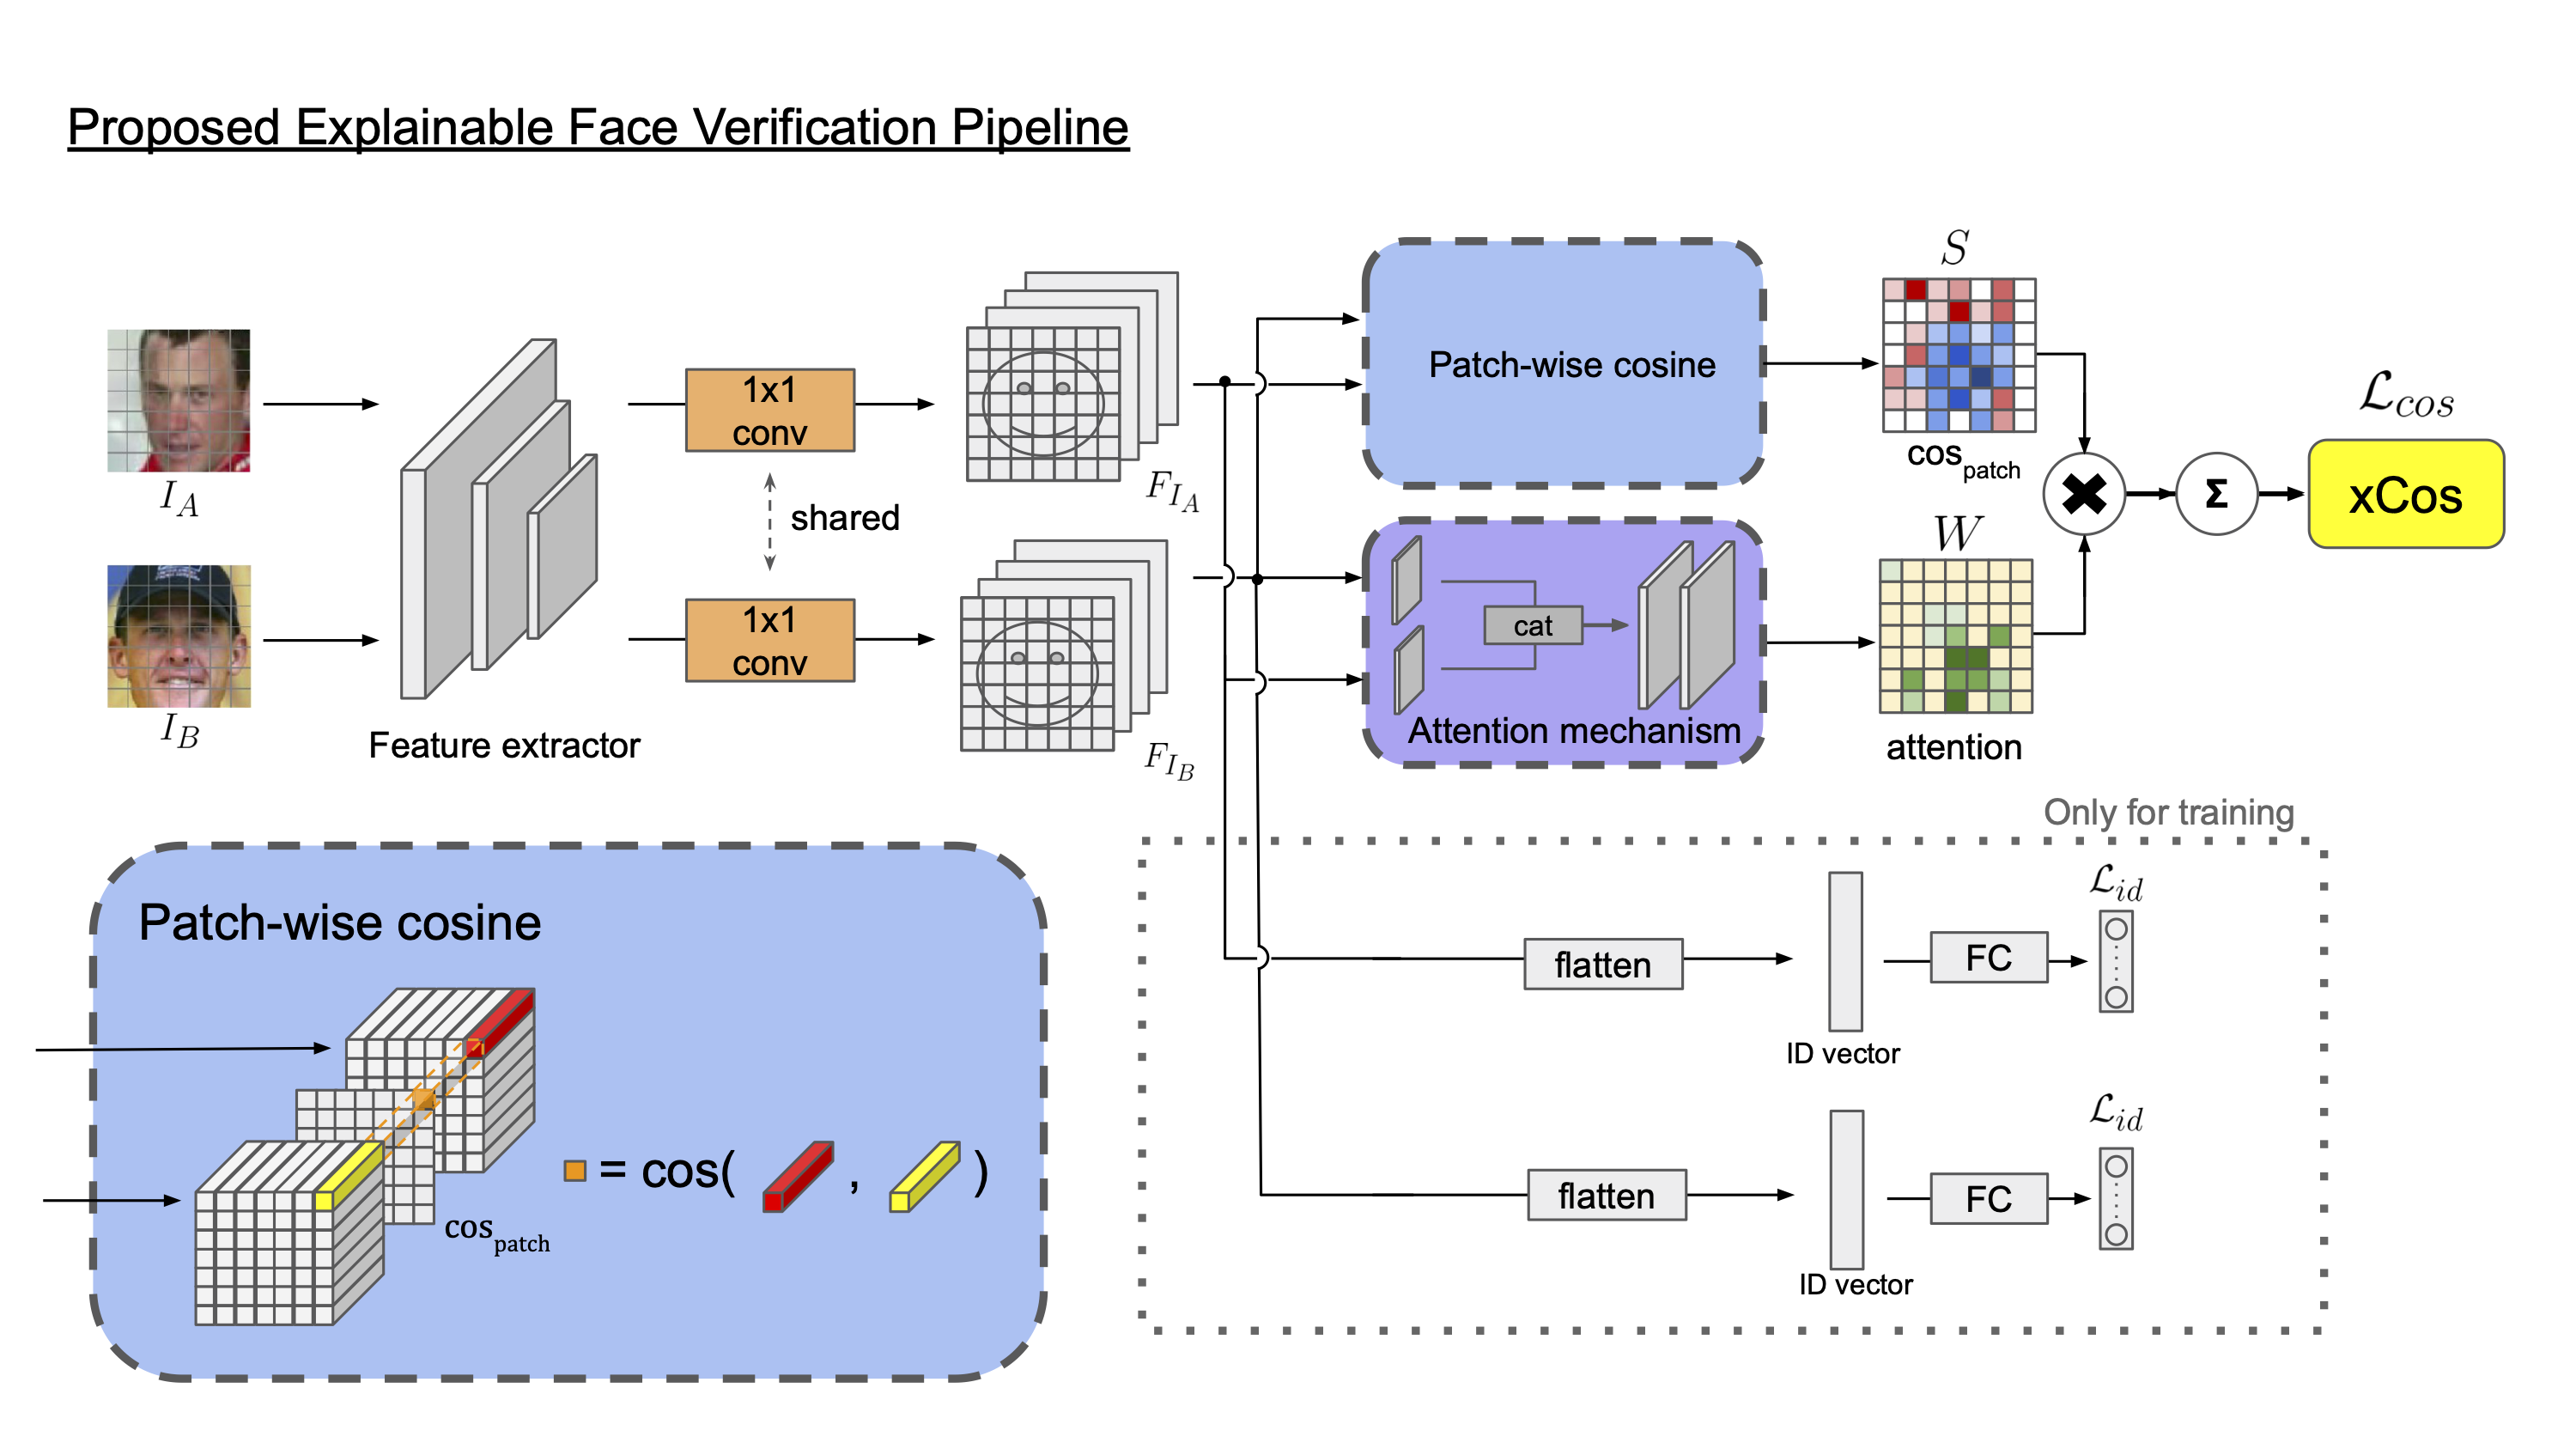
\includegraphics[scale=0.5]{figures/xCos-architecture.png}
  \caption{Example of the xCos architecture taken from~\cite{xCos}}
  \label{fig:xCos architecture}
\end{figure}

\subsubsection{Fréchet Inception Distance}